\documentclass{article}
\usepackage{color}
\usepackage{here}
\usepackage{url}
\usepackage[dvipdfmx]{graphicx}
\usepackage{graphicx}
\usepackage[dvipdfmx]{hyperref}
\usepackage{hyperref}


\title{A comparison of different meshing algorithms}

\begin{document}

\maketitle 
\section{Implicit surface meshing}
In order to obtain a deformed surface, we need to compute a triangle mesh approximation of the implicit surface computed from the deformed point-cloud (given by the deformed mesh vertices). The following meshing algorithms are considered: the Marching Cubes algorithm \cite{LC87}, a Delaunay-based meshing algorithm (which is a modification of the algorithm described in \cite{FP12}), and the CGAL implementation (see \cite{RY07, CGAL}) of the implicit surface meshing algorithm \cite{BO05}.

% ref are missing for these algos
In the following descriptions, we assume that $f$ is a given trivariate function obtained from an implicit surface reconstruction algorithms. We used Hermite Radial Basis Function (HRBF) and Poisson surface reconstruction. 
Let $P$ be the point-cloud obtained from the deformed vertices of the input surface.

\subsection{The Marching Cubes algorithm}
The Marching Cubes algorithm is an algorithm for rendering isosurfaces from volumetric data. The basic idea is to consider a bounding box for the object to be meshed (corresponding to $f=0$) and to subdivide it regularly into smaller cells. 
The function $f$ is then sampled at the eight corners of each cell. If one or more values is less than the user-specified isovalue (we use $0$), and one or more values is greater than this isovalue, the cell must intersect the surface. By determining the edges in the cell that are intersected by the surface, and connecting them we can form a linear approximation of the surface in each cell. By connecting the patches from all cells, we get a linear approximation of the isosurface.
Note that in this algorithm, we do not use the information provided by the point-cloud $P$.
 
\subsection{Delaunay based implicit surface meshing}
Since we know that all the points from the deformed point-cloud $P$ belong to the surface of the deformed object (or at least are close to it), Marching Cubes based algorithm do not look like the most effective approach. Instead one could compute a Delaunay tetrahedralization of the deformed point-cloud and peel off outside tetrahedra using the function $f$. This is a simple modification of the algorithm described in \cite{FP12}, except that we do not need to sample from the surface, but use the samples from $P$ instead.

\subsection{The CGAL implicit surface mesher}
An alternative is the CGAL implementation of the implicit surface meshing algorithm of Boissonnat and Oudot \cite{BO05}.
The CGAL implementation can also start from the samples in $P$, which helps decreasing the running time of the algorithm. However, in order to maintain guarantees on the generated triangle mesh, the algorithm performs additional sampling of the implicit surface, as well as additional computations. 


\section{Computational complexity}
\label{sec:mesh_comp_time}
We now turn to a brief asymptotic analysis of the time complexity of these different meshing algorithms. 
The following quantities will be used: $v$ the number of points in the input point-cloud $P$, 
and $n$ the resolution (along one direction) of the regular grid used by the Marching Cubes algorithm.

We are only interested in the time complexity for generating the mesh (and ignore the time complexity for constructing $f$). 
This is given by the cost of the evaluation of $f$ multiplied by the number of evaluation. 
Two reconstruction methods are considered: 
HRBF, which has a complexity $O(v)$, and Poisson surface reconstruction, which has a complexity of $O(v^{1/3})$.
 
For Poisson surface reconstruction, we are using the CGAL implementation. In this implementation, the evaluation of $f$ at a given point is done by locating the tetrahedron containing the point, and using interpolation of the values specified at the tet's nodes, by barycentric coordinates. The complexity for evaluating $f$ in this case, is thus equal to the complexity for locating a tetrahedron containing a query point in a $3D$ Delaunay triangulation. CGAL implementation uses a random walk algorithm with complexity $O(v^{1/3})$. 
\\
Remark: The $3D$ Delaunay triangulation used for solving the Poisson problem in the Poisson surface reconstruction approach, contains more than $v$ vertices, since Steiner point are added. However, the number of added Steiner points is in the same order of magnitude, thus complexity above remains valid.

\subsection{The Marching Cubes algorithm}
Based on the previous analysis, the asymptotic time complexity for the Marching Cubes algorithm is:
\begin{itemize}
\item $O(n^3 \; v)$ when HRBF is used;
\item $O(n^3 \; v^{1/3})$ when Poisson surface reconstructio is used.
\end{itemize}

\subsection{Delaunay-based meshing}
For determining the complexity of the Delaunay based mesher, we need to determine the number of tetrahedra in a $3D$ Delaunay triangulation. 
The number of simplices in the worst case is $O(v^2)$. 
However, a paper by Attali and Boissonnat \cite{AB04} suggests that the number of simplices in a $3D$ Delaunay triangulation is actually linear, when the points are sampled on the surface of an object.
Thus, we should expect in practice a complexity of $O(v^2)$ when HRBF is used, and $O(v^{4/3})$ when Poisson surface reconstruction is used.

\subsection{CGAL implicit surface mesher}
It is difficult to determine the time complexity of the implicit surface mesher implemented in CGAL, 
because the algorithm is iterative, and adds more samples on the surface based on several conditions. 


\section{Numerical experiments}
\label{sec:mesh_exp}
We turn now to numerical experiments to determine the running time of these different meshing algorithms, when combined with an implicit surface reconstruction algorithm.

Points sampled on unit sphere are prepared with the following method:
given an implicit definition of a unit sphere, we compute a triangle mesh approximation using the Marching Cubes algorithm. We use different grid resolutions, in order to create triangle meshes with different number of vertices and triangles. These triangle meshes will be used as the input data for comparing the different meshing algorithms after fitting an implicit surface.

The three different meshing algorithms compared are:
\begin{itemize}
\item The Marching Cubes algorithm; 
\item The Delaunay-based meshing algorithm; 
\item The implicit surface meshing algorithm of CGAL.
\end{itemize}

These meshing algorithms are applied to a function $f$ obtained either by the Poisson surface reconstruction algorithm or by fitting a compactly supported Hermite Radial Basis Function (HRBF).
Overall, we are expecting the Delaunay based surface mesher to be the most efficient, because we already have a sampling of the surface to start with. By comparison the Marching Cubes algorithm needs to always sample the reconstructed function on a regular grid, which can be expensive if the grid has a high resolution.
The CGAL implicit surface mesher is using a more sophisticated sampling algorithm to probe the surface, and is thus relatively expensive. When using the CGAL surface mesher in the experiments below, we use as an input sampling of the surface the points from the input point-cloud.

Tables \label{hrbf_16} to \label{Pois_256} below show the running time obtained by the different meshing algorithms for reconstructing a unit sphere from point-clouds of different sizes.

\begin{table}
 \caption{HRBF reconstruction and meshing from a sphere with 480 vertices and 956 faces. The input mesh was obtained with the Marching Cubes algorithm using a grid resolution of $16^3$.}
\label{hrbf_16}
  \begin{tabular}{|l|c|c|c|} \hline
    Meshing algorithms & Marching Cubes & Delaunay & CGAL \\  \hline
    Time [ms] & 40 & 30 & 4936\\ \hline
    $\sharp$ vert., $\sharp$ faces & 552, 1096 & 480, 954 &2102, 4196 \\ \hline
  \end{tabular}
\end{table}

\begin{table}
 \caption{Poisson surface reconstruction and meshing from a sphere with 480 vertices and 956 faces. The input mesh was obtained with the Marching Cubes algorithm using a grid resolution of $16^3$}
\label{Pois_16}
  \begin{tabular}{|l|c|c|c|} \hline
    Mesh algorithms & Marching Cubes & Our Delaunay & CGAL Delaunay \\  \hline
    Time [ms] & 7 & 25 & 1034\\ \hline
    $\sharp$ vert., $\sharp$ faces & 480, 956 & 480, 930 &1719, 3434 \\ \hline
  \end{tabular}
\end{table}

\begin{table}
 \caption{HRBF reconstruction and meshing from a sphere with 1992 vertices and 3980 faces. The input mesh was obtained with the Marching Cubes algorithm using a grid resolution of $32^3$.}
\label{hrbf_32}
  \begin{tabular}{|l|c|c|c|} \hline
    Mesh algorithms & Marching Cubes & Our Delaunay & CGAL Delaunay \\  \hline
    Time [ms] & 646 & 80 & 21669\\ \hline
    $\sharp$ vert., $\sharp$ faces & 2736, 5464 & 1992, 3970 &4769, 9530 \\ \hline
  \end{tabular}
\end{table}

\begin{table}
 \caption{Poisson surface reconstruction and meshing from a sphere with 1992 vertices and 3980 faces. The input mesh was obtained with the Marching Cubes algorithm using a grid resolution of $32^3$}
\label{Pois_32}
  \begin{tabular}{|l|c|c|c|} \hline
    Mesh algorithms & Marching Cubes & Our Delaunay & CGAL Delaunay \\  \hline
    Time [ms] & 40 & 87 & 2118\\ \hline
    $\sharp$ vert., $\sharp$ faces & 2004, 4004 & 1992, 3628 &3887, 7766 \\ \hline
  \end{tabular}
\end{table}

\begin{table}
 \caption{HRBF reconstruction and meshing from a sphere with 8376 vertices and 16748 faces. The input mesh was obtained with the Marching Cubes algorithm using a grid resolution of $64^3$.}
\label{hrbf_64}
  \begin{tabular}{|l|c|c|c|} \hline
    Mesh algorithms & Marching Cubes & Our Delaunay & CGAL Delaunay \\  \hline
    Time [ms] & 24407 & 360 & 622310\\ \hline
    $\sharp$ vert., $\sharp$ faces & 13944, 27880 & 8376, 16754 &21143, 42274 \\ \hline
  \end{tabular}
\end{table}

\begin{table}
 \caption{Poisson surface reconstruction and meshing from a sphere with 8376 vertices and 16748 faces. The input mesh was obtained with the Marching Cubes algorithm using a grid resolution of $64^3$.}
\label{Pois_64}
  \begin{tabular}{|l|c|c|c|} \hline
    Mesh algorithms & Marching Cubes & Our Delaunay & CGAL Delaunay \\  \hline
    Time [ms] & 221 & 256 & 16276\\ \hline
    $\sharp$ vert., $\sharp$ faces & 8378, 16752 & 8376, 14665 &20876, 41748 \\ \hline
  \end{tabular}
\end{table}

\begin{table}
 \caption{Poisson surface reconstruction and meshing from a sphere with 33696 vertices and 67388 faces. The input mesh was obtained with the Marching Cubes algorithm using a grid resolution of $128^3$.}
\label{Pois_128}
  \begin{tabular}{|l|c|c|c|} \hline
    Mesh algorithms & Marching Cubes & Our Delaunay & CGAL Delaunay \\  \hline
    Time [ms] & 1332 & 1133 & 73303\\ \hline
    $\sharp$ vert., $\sharp$ faces & 33696, 67388 & 33696, 55877 &76641, 153278 \\ \hline
  \end{tabular}
 \end{table} 
 
\begin{table}
 \caption{Poisson surface reconstruction and meshing from a sphere with 136224 vertices and 272444 faces. The input mesh was obtained with the Marching Cubes algorithm using a grid resolution of $256^3$.}
\label{Pois_256}
  \begin{tabular}{|l|c|c|c|} \hline
    Mesh algorithms & Marching Cubes & Our Delaunay & CGAL Delaunay \\  \hline
    Time [ms] & 9763 & 3695 & 408205\\ \hline
    $\sharp$ vert., $\sharp$ faces & 136222, 272440& 136224, 185169 &343567, 686970 \\ \hline
  \end{tabular}
\end{table}

We remark in the previous tables that the number of vertices (and faces) is higher than the expected number of vertices (for a given the grid resolution), when the Marching Cubes algorithm is used to mesh the function obtained from HRBF fitting.
The problem comes from the fact that compactly supported splines are used, and they create additional zero isosurfaces away from the object surface. It is not difficult to modify the Marching Cubes algorithm in order to ignore these extra surfaces. However, this does not impact much the running time of the Marching Cubes, since the bottleneck is in sampling the function on the regular grid. Therefore, we did not write additional code to ignore these extra surfaces.

\begin{figure}[h]
\begin{center}
\caption{Marching Cubes, Our Delaunay and CGAL Delaunay time}
 \label{fig:threegraph}
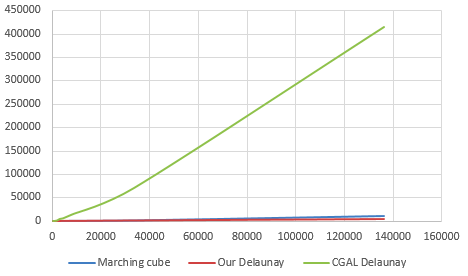
\includegraphics[width=10cm]{compare_mesher_graph.png}
\end{center}
\end{figure}

\begin{figure}[h]
\begin{center}
\caption{Our Delaunay and CGAL Delaunay time}
 \label{fig:twograph}
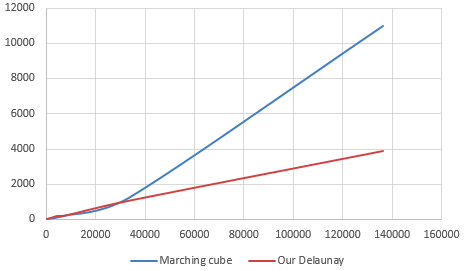
\includegraphics[width=10cm]{marching_and_delaunay_timegraph.png}
\end{center}
\end{figure}

Figures \ref{fig:threegraph} and Figure \ref{fig:twograph} show plots of the running time in milliseconds for the three different meshing algorithms, when the Poisson surface reconstruction method is used. 
The horizontal axis corresponds to the number of points in the input point-cloud.
The vertical axis gives the running times for the input of different sizes.


\section{Conclusion}
The preliminary analysis (Section \ref{sec:mesh_comp_time}) and the numerical experiments (Section \ref{sec:mesh_exp}) seem to indicate that the Delaunay-based meshing algorithm is preferable for our use case.
In addition to being slower for our particular case, the Marching Cubes algorithm has the following disadvantages over the Delaunay based implicit surface meshing algorithms:
\begin{itemize}
\item It generates poor shaped triangle;
\item It is difficult to estimate the grid resolution to use in order to maintain approximately the number of vertices on the surface.
\end{itemize}


%%%%%%%%%%%%%%%%%%%%%%%%%%%%%%%%%%%%%%%%%%%%%%%%%%%%%%%%%%%%%%%%%%%%%%%%%%%%%%%%%%%%%%%%%%

\begin{thebibliography}{9}
\bibitem{LC87}
William E. Lorensen and Harvey E. Cline. Marching Cubes: A high resolution 3D surface construction algorithm. SIGGRAPH Comput. Graph. 21, 4 (August 1987), 163-169.

\bibitem{FP12}
Pierre-Alain Fayolle and Alexander Pasko. Optimized surface discretization of functionally defined multi-material objects. Adv. Eng. Softw. 45, 1 (March 2012), 301-312.

\bibitem{BO05}
Jean-Daniel Boissonnat and Steve Oudot. Provably good sampling and meshing of surfaces. Graphical Models, 67:405-451, 2005.

\bibitem{RY07}
Laurent Rineau and Mariette Yvinec. A generic software design for Delaunay refinement meshing. Comput. Geom. Theory Appl., 38:100-110, 2007.

\bibitem{AB04}
Dominique Attali and Jean-Daniel Boissonnat. A linear bound on the Complexity of the Delaunay Triangulation of Points on Polyhedral Surfaces. INRIA Technical report. 2004.

\bibitem{CGAL}
CGAL 4.9.1 - 3D Surface Mesh Generation \\
\url{http://doc.cgal.org/latest/Surface_mesher/group__PkgSurfaceMesher3FunctionsMakeMesh.html}
\end{thebibliography}

%%%%%%%%%%%%%%%%%%%%%%%%%%%%%%%%%%%%%%%%%%%%%%%%%%%%%%%%%%%%%%%%%%%%%%%%%%%%%%%%%%%%%%%%%%

\end{document}
